% Chapter ApnaService

\chapter{APNA as SCION Service} % Main chapter title

\label{apna_service}
In this chapter we will discuss the third approach to implement a new APNA as a SCION service. This chapter is structured as follows: \ref{ser:main_idea} covers the core idea behind this approach and describes the interaction with the APNA service, followed by Section \ref{srv:mod} which discusses the technical difficulties and the modifications required in the current infrastructure. Section \ref{srv:comm} presents an example in which two host communicate using the new address family. In the end we will discuss the drawback related to this approach \ref{srv:draw}. 

\section{Main Idea} \label{ser:main_idea}
APNA Service (\texttt{AP\_SVC}) approach is radically different from the past two approaches described in previously i.e., APNA over SCION (Chapter \ref{apna_overlay}) and APNA address family (Chapter \ref{address_family}). The main idea behind this approach is to create a new SCION service (such as Path Service, Certificate Service) which would be responsible for forwarding APNA packets. The main advantage of this approach instead of modifying the border router and dispatcher to handle APNA packets this new service will take care of APNA packets instead. That makes this approach easily deploy-able on the current SCIONLab infrastructure without a lot of changes in the existing deployment.

APNA service is like a data plane service which is responsible for providing anonymous communication service for SCION. Any packet send to APNA service will get anonymously delivered to the destination. Source APNA service uses the anycast address to deliver the packet to destination APNA service which then forwards it to the appropriate host. Since we are using the anycast address for communication attacker cannot hamper the anonymity guarantees provided by APNA framework. APNA service consists of two different services inside it:
\begin{itemize}
    \item IP-UDP based service for the host to send packets to it.
    \item SCION-UDP based service for sending packets to another APNA service.
\end{itemize}
We require two different services is because of the limitation of current SCION SNET API as it does not allow sending packets to service inside same \texttt{ISD-AS}.

\subsection{APNA Service Architecture}
\paragraph{Design Goals for APNA service}
APNA Service needs to be highly reliable and efficient and in order to achieve this goal, its designed as a highly concurrent service using go-routines. Each functionality of APNA Service is distributed among different go-routines in order to avoid bottlenecks and use the power of multiprocessing to the full extend. There are multiple go-channels and each channel has a go-routine associated with it and whenever a packet arrives it gets processed by the appropriate go-routine and forwarded to the next channel for further processing.

\subsection{Processing Outgoing Packet by APNA Service} \label{apna_service:out}
Firstly APNA Service reads the packet from the \textit{UDP} network socket and transfers that packet to the receive queue. Another go-routine will read packet from this receive queue and try to serialize the packet and if the serialization is successful it will be put into MAC Verification Queue. Otherwise it will be forwarded to error queue and a SCMP message will be sent to the sender of the packet.

If the packet reaches MAC verification queue another go-routine would perform MAC verification for the packet. If the packet has not been tampered then the MAC verification would succeed and forwarded to the forwarding queue. Otherwise packet would be dropped.

Forwarding queue go-routine would try to de-serialize the packet so that it could be forwarded to the border router which could deliver the packet to the destination. But if there is a error while de-serializing the packet and it would be moved to error queue and eventually a SCMP message will be sent to sender.
\begin{figure}[th!!]
\centering
\hspace*{-2cm}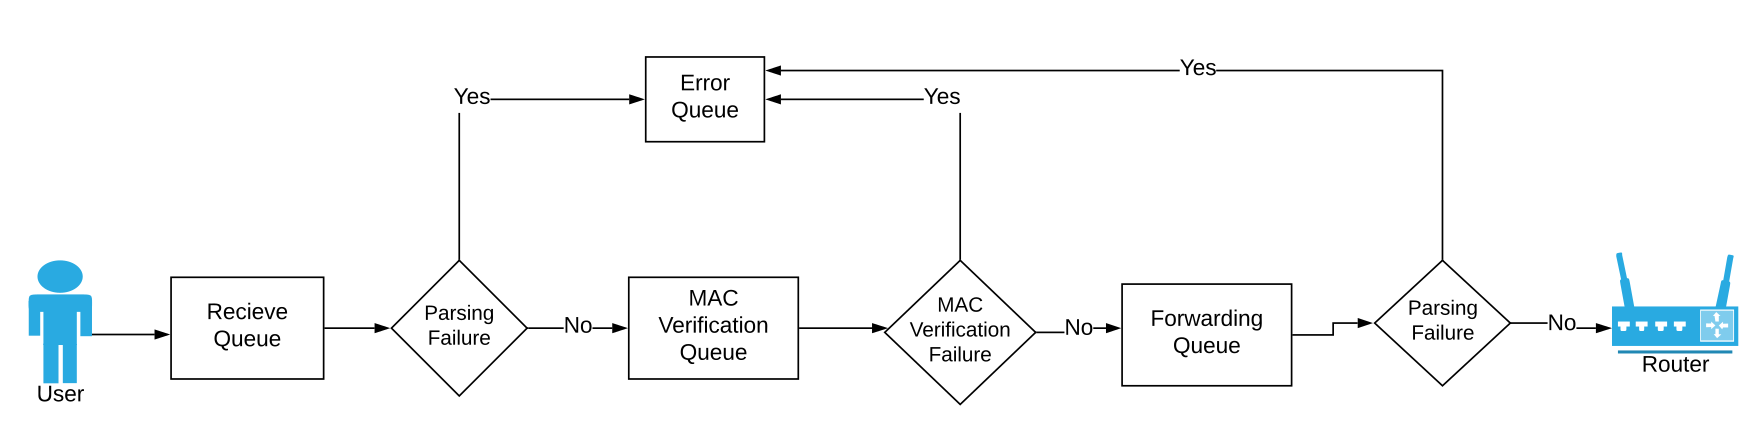
\includegraphics[scale=0.3]{Figures/svc.png}
\decoRule
\caption[APNA Service Outgoing Packet]{Outgoing Packet Processing by APNA Service}
\label{fig:apna_svc_out}
\end{figure}

\subsection{Processing Incoming Packet by APNA Service}  \label{apna_service:in}
\begin{figure}[th!!]
\centering
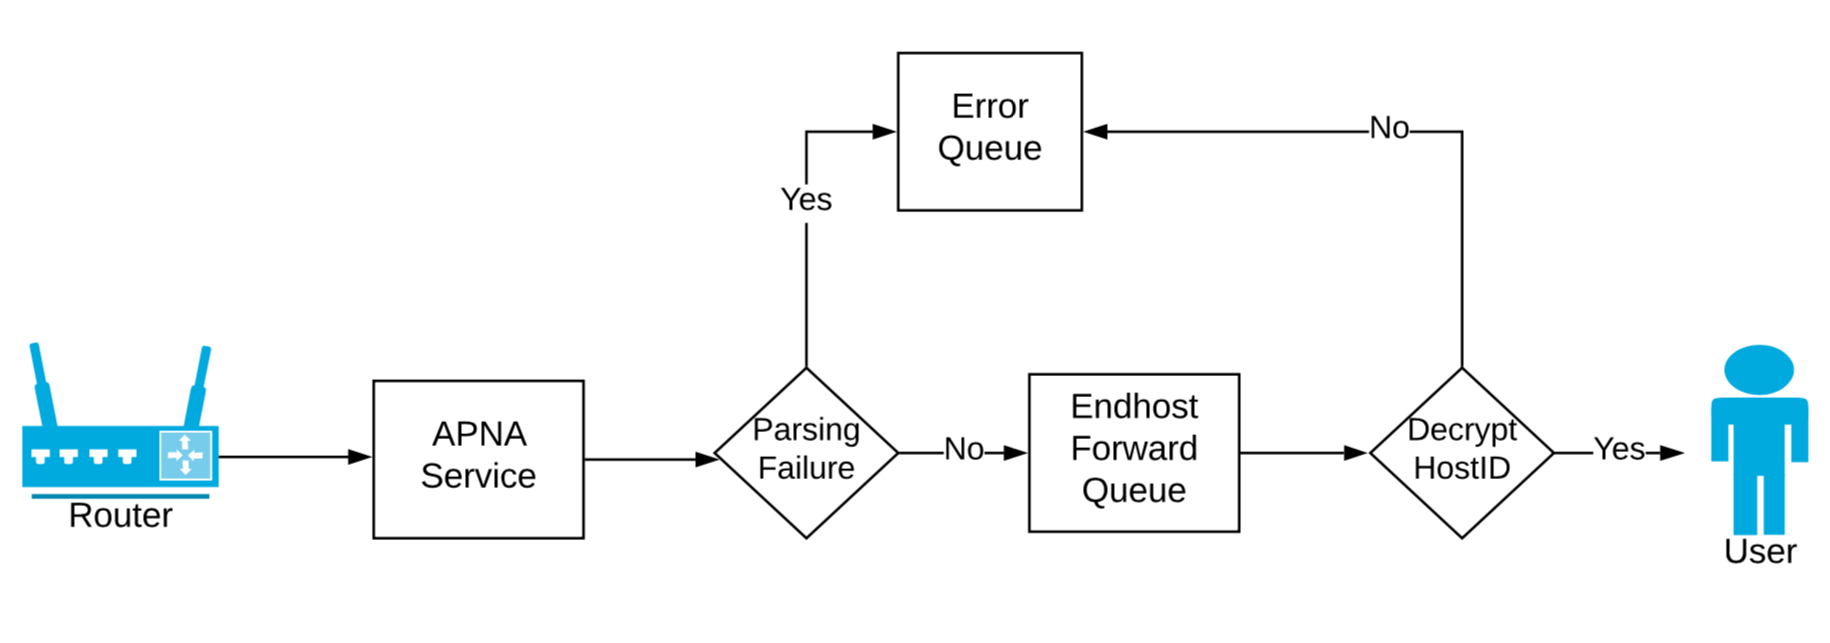
\includegraphics[scale=0.24]{Figures/svc_out.png}
\decoRule
\caption[APNA Service Incoming Packet]{Incoming Packet Processing by APNA Service}
\label{fig:apna_svc_in}
\end{figure}
Figure \ref{fig:apna_svc_in} represents a scenario how does a APNA service processes an incoming packet? In the first step APNA service will parse the packet, if successful it will transfer the packet to \texttt{EndhostForwardQueue} else it would be moved to \texttt{ErrorQueue} and eventually gets dropped. \texttt{EndhostForwardQueue} goroutine will decrypt the EphID to obtain HID and after that contact IMS to convert HID to IP address to forward the packet to the destination endhost using a UDP socket.

\subsection{APNA Service Request Packet Format}
\begin{figure}[th!!]
\centering
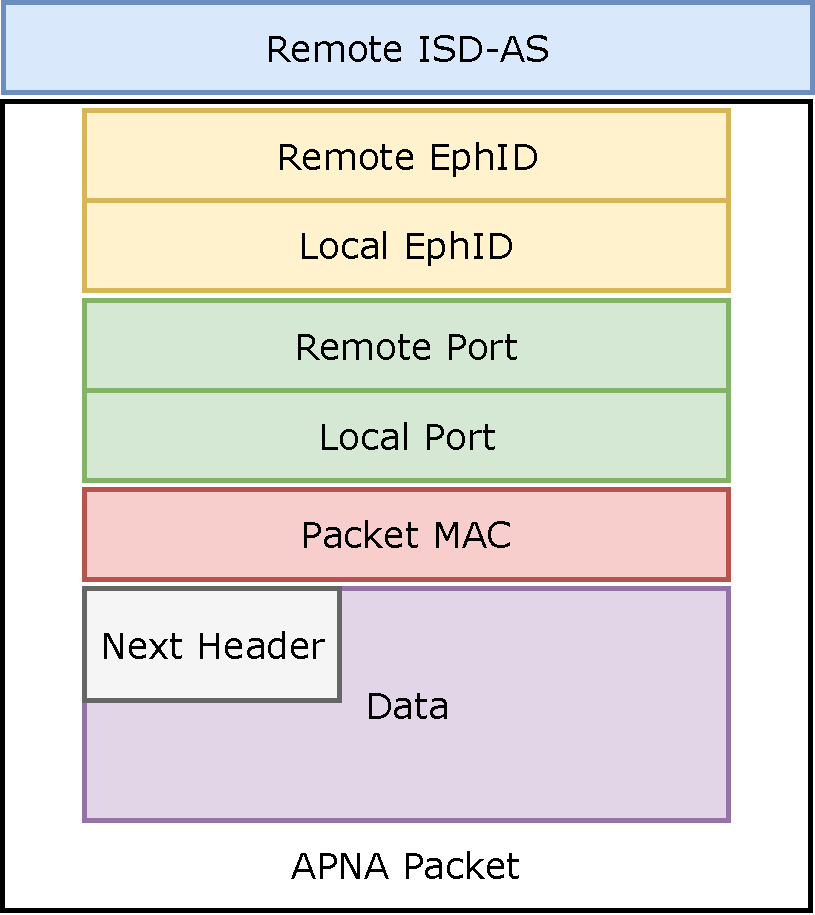
\includegraphics[scale=0.6]{Figures/apna_svc_request_pkt.pdf}
\decoRule
\caption[APNA Service Incoming Packet]{APNA Service incoming packet}
\label{fig:apna_svc_request_pkt}
\end{figure}
APNA service is a \texttt{UDP} based service and the host which want to use APNA service they need to send packets in the certain format so that APNA service can construct a SCION-APNA packet out of it and send it to the service on the destination side. This packet structure contains lots of information which will be present inside SCION header but since its a based service it does not have all that information. SCION packet will be constructed using this packet.

This is can be simplified if SNET API allows host to send packet to service using its anycast service address. This issues has been reported to SCION team and they will take care of it in the near future. 

\section{Modifications in the current infrastructure} \label{srv:mod}
There are various reason which attribute for adjustment in the current SCION infrastructure to introduce a new service address for APNA service.

\begin{itemize}
    \item Since there is no service discovery implemented inside SCION currently so all the application which needs to perform translation from service address to overlay IP address will need modifications.
    \item SCIOND needs to extended to be able to translate service address to IP address for the endhosts.
    \item Userspace SNET APIs need to changed to send packets to APNA service instead of next hop border router.
\end{itemize}

\subsection{Border Router}
Unlike previous approach border routers do not need to be changed as significantly. As most of the functionality related verifying packet authenticity is offloaded to APNA service.

The only change that is required in the BR is at the destination BR packet processing to handle new APNA service address (\texttt{SvcAP}). Border routers usually find the IP address of the service by parsing the \texttt{topology.json} and once its updated it can handle the new service address. Listing \ref{code:apna_svc} shows the portion that needs to be added inside border router's \texttt{topology.json}

\begin{code}
\captionof{listing}{Extension for BR topology.json}
\inputminted[frame=lines, framesep=2mm, baselinestretch=1.2, fontsize=\footnotesize, linenos]{json}{code_snippets/apnasvc.json} \label{code:apna_svc}
\end{code}

\subsection{SNET}
SCION initialization phase needs to be modified. It needs to contact SCIOND and establish a UDP connection with APNA service which can be used later to send packet APNA service.

SNET needs to provide an interface to interact with APNA service namely a read and write interface. It also needs to resolve the IP address associated with APNA service for that \texttt{ISD-AS}. SNET provides two new API
\begin{itemize}
    \item \texttt{snet.ReadAPNA()} \\
    In the background it reads from the UDP connection established with APNA service during the initialization phase and read the APNA packet inside a buffer. At last that buffer is forwarded to the endhost.
    \item \texttt{snet.WriteAPNA()} \\
    Behind the scenes this function uses the connection established with APNA service during the initialization phase and forward the packet to APNA service
\end{itemize}

These two new functions are provided on the same \texttt{snet.Conn} interface.

\subsection{SCIOND}
As discussed in Section \ref{background:sciond} \texttt{SCIOND} is responsible for service address resolution as well. Thus \texttt{SCIOND} needs to be extended for the same reason for new APNA service. All the endhost use the IP address provided by SCIOND to send packets and receive packets from APNA service.

Currently there are two different implementation of SCIOND Python and Golang. But in the production mostly Python version is in use but in order to be ready for future versions of SCION both implementation needs to be extended.

\texttt{CapnProto} specification for SCIOND also needs to be extended to introduce new \texttt{SvcAP} address type. Anycast address assigned to APNA service is (0x0004). 

\subsection{SCION-APNA Packet Structure}
Figure \ref{fig:apna_svc_pkt} represents the packet structure used by APNA service to communicate with each other. It encapsulates the APNA packet inside it. We need add port information inside APNA packet since there is no port information is required to forward the packet to the endhost.
\begin{figure}[th!!]
\centering
\noindent
\makebox[\textwidth]{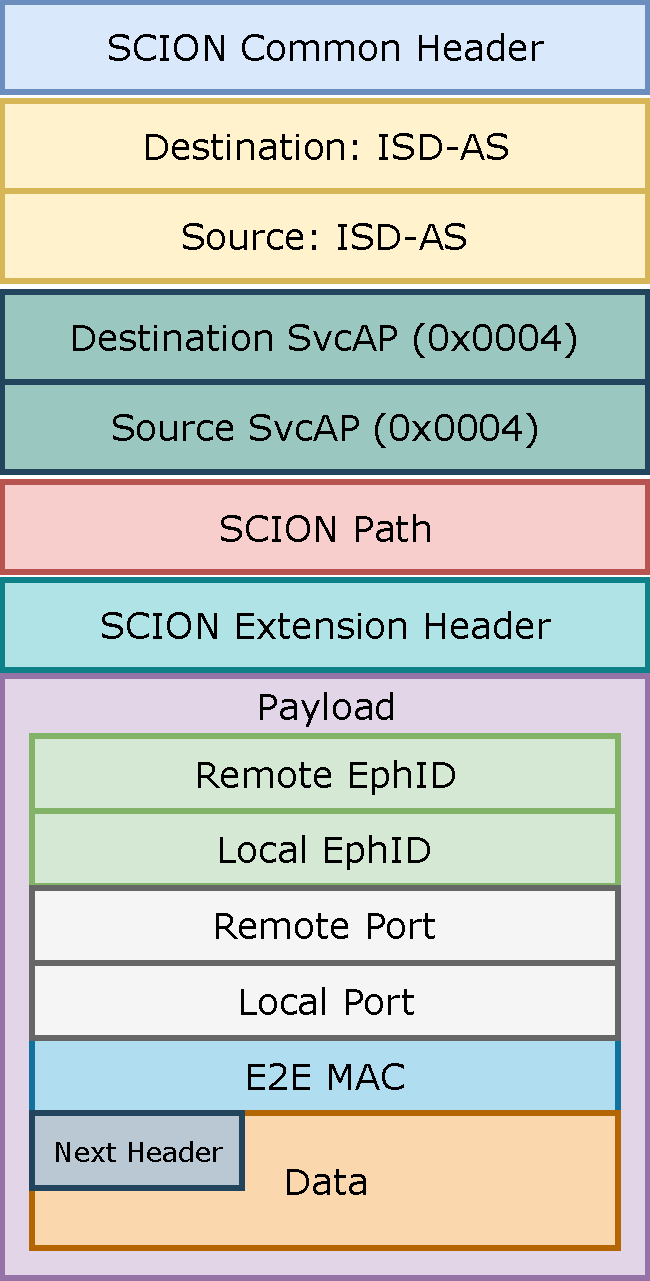
\includegraphics[scale=0.6]{Figures/apna_svc.pdf}}
\decoRule
\caption[APNA packet structure using SvcAP]{APNA packet structure  using SvcAP for forwarding APNA packets}
\label{fig:apna_svc_pkt}
\end{figure}


\section{Data Communication} \label{srv:comm}
\begin{figure}[th!!]
\centering
\hspace*{-1cm}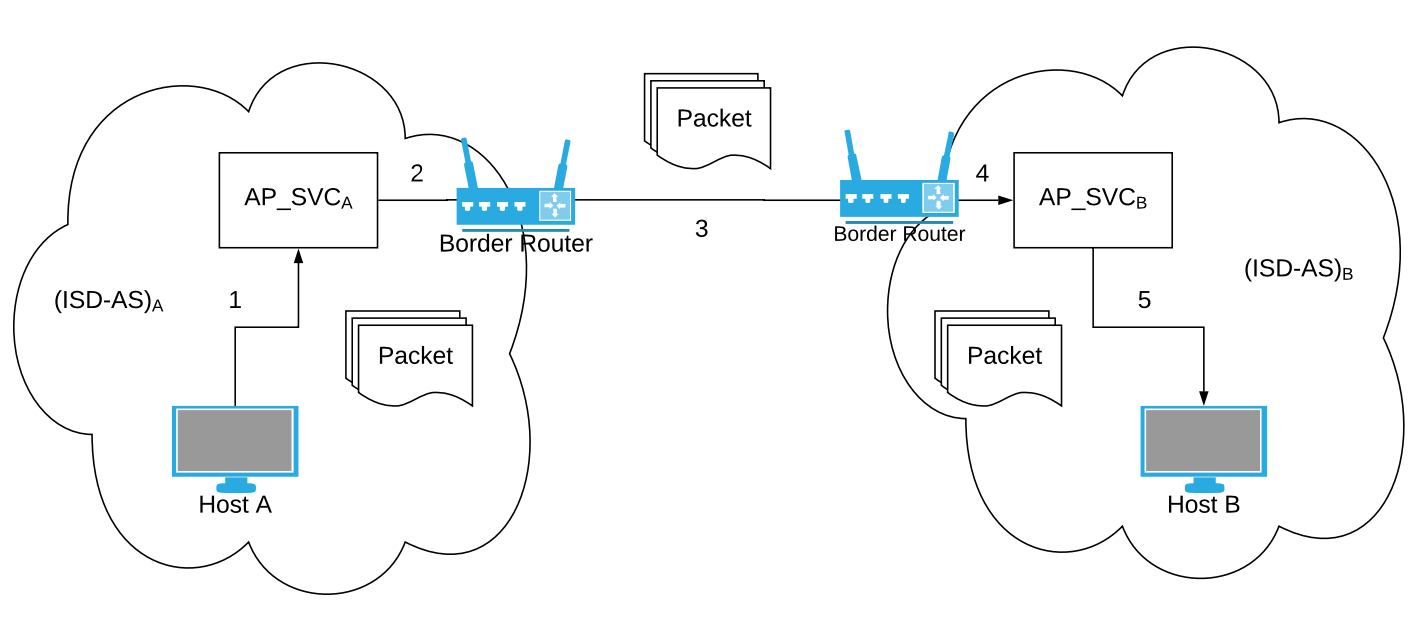
\includegraphics[scale=0.35]{Figures/svc_arch.png}
\decoRule
\caption[Communication overview for APNA Service]{Communication overview for APNA Service architecture}
\label{fig:srv_comm}
\end{figure}
Figure \ref{fig:srv_comm} represents a simple scenario in which two host can communicate with each other using this new APNA service. In this case Host A which is located in \texttt{(ISD-AS)}$_A$ wants to send a packet to Host B located in \texttt{(ISD-AS)}$_B$. It can be broken down into five steps as show in the figure. 

\subsection{Part One: Establish comm. and send packet to APNA service}
Initially the host needs to initialize the SCION networking context and use DNS service to obtain the EphID associated with Host B. After that Host A creates a APNA service request packet as described in Figure \ref{fig:apna_svc_request_pkt} and using the SNET's API it forwards the packet to APNA service in the same \texttt{ISD-AS}. 

\subsection{Part Two: APNA service process packet and forward it to BR}
After receiving the packet APNA service processes the packet as described in Section \ref{apna_service:out} and using the path service finds the path to APNA service at the destination host. After that it can simply construct a new SCION packet by de-capsulating APNA packet from APNA service packet and use that as the payload for the newly constructed SCION packet as shown in Figure \ref{fig:apna_svc_pkt}. 

\subsection{Part Three: Intra domain routing among BR}
Border routers can forwards the APNA service packet just like a normal SCION service packet using the path information present inside the packet.

\subsection{Part Four: Destination BR forward packet to APNA service}
At the last hop border router it will notice the anycast service address in the SCION packet. In order to forward that packet border router needs to convert that anycast address to an IP address. IP address can be obtained from the \texttt{topology.json} which was passed an argument to border router when it was started.

\subsection{Part Fifth: APNA service delivering packet to destination host}
In order to forward the packet to the destination host APNA service requires two think an IP address and a port number. Destination port number is already present inside the APNA service request packet. In order to obtain IP address from destination EphID APNA service can use the same algorithm previously used by destination border routers. The whole process how the APNA service process a outgoing packet is explained in the Section \ref{apna_service:in}.

\section{Drawbacks} \label{srv:draw}
The main drawback behind this approach it increases the header size as EphID and Port number are pushed back into payload. And it requires modification the whole build and deployment system to introduce a new service in the SCION infrastructure.

\section{Comparison between all three approaches}
\bgroup
\def\arraystretch{1.5}%
\begin{center}
\captionof{table}{Comparison between all three different approaches to implement APNA inside SCION} \label{tab:notation} 

\begin{table}[th!!]
\begin{tabular}{|c|c|c|c|}
\hline
                                                                           & \textbf{Approach 1}                                                                                          & \textbf{Approach 2}                                                                                       & \textbf{Approach 3}                                                                                                                   \\ \hline
\textbf{\begin{tabular}[c]{@{}c@{}}SCIONLab \\ Deployability\end{tabular}} & Possible                                                                                                     & Not Possible                                                                                              & Possible                                                                                                                              \\ \hline
\textbf{\begin{tabular}[c]{@{}c@{}}Implementation \\ Efforts\end{tabular}} & \begin{tabular}[c]{@{}c@{}}Major modifications \\ in source \\ and destination \\ border router\end{tabular} & \begin{tabular}[c]{@{}c@{}}Major modifications \\ in all the border \\ router and dispatcher\end{tabular} & \begin{tabular}[c]{@{}c@{}}New SCION service\\ implementation with minor \\ modifications in \\ border router and SCIOND\end{tabular} \\ \hline
\textbf{MTU}                                                               & 1336                                                                                                         & 1378                                                                                                      & 1320                                                                                                                                  \\ \hline
\end{tabular}
\end{table}
\end{center}
\egroup

In the end we finally deployed approach 3 on the SCIONLab infrastructure since it required minimum modifications in the existing SCION infrastructure. This approach even helps in the future when we want to make modifications inside the existing APNA protocol it would be much easier to do because of reducing coupling the SCION infrastructure. 